% Chapter 2 of the Thesis Template File
%   which includes bibliographic references.
\chapter{REVIEW OF LITERATURE}
In this chapter, we will overview main differences between NL versus PL and understand meaning of each natural language elements. To get this summarization of problems between two languages, we rely on problems between NL and PL listed in [\cite{Pulido-Prieto:2017:SNP:3145473.3109481}] and problems we found.
\section{Differences between Natural Language and Programming Language}
According to [\cite{Pulido-Prieto:2017:SNP:3145473.3109481}], programming language has limit language expressiveness while natural language description has stronger expressiveness.  In natural language, there are linguistic elements that have a different level of expressiveness compare to programming language.
\subsection{Deixis}
According to Oxford English Dictionary, "deixis" means "the function or use of deictic words or expressions whose meaning depends on where, when, or by whom they are used". In other words,this concept highlight that in natural language, there are words that their meaning depend on the context. Deixis are used to express the sentence in  shorter way without losing its meaning. In the direction of NL to PL, along with the context of NL, we have the context from the surrounding source code. \\

\begin{figure}[htp]
	\centering
	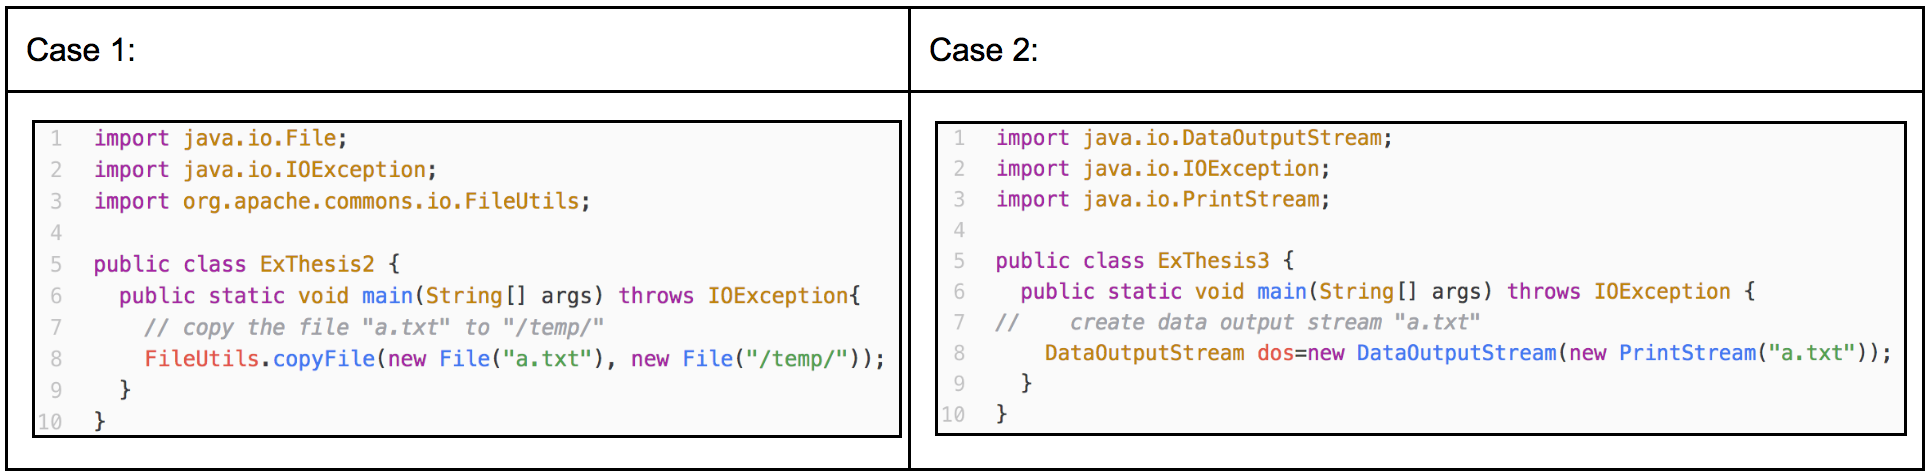
\includegraphics[width=17cm,height=6cm]{resources/fig_deixis_example.png}%
	%\includegraphics[width=\textwidth]{conceptdriven.eps}
	\caption[Example of Deixis in NL-to-PL translation]{Example of Deixis in NL-to-PL translation} 
	\label{fig:DeixisExample}
\end{figure}

An example of deixis is shown in the code snippet in Figure \ref{fig:DeixisExample}. In this example, "the file" here has the reference to the type "java.io.File". In this context, although the description mentioned only about a class name. There are several ways for describe an object by deixis, like using pronouns such as "it" or "they". In the other words, deixis provides a type of indirect reference between object in natural language and object in implementation. \\

Another example is case 2 in figure \ref{fig:DeixisExample}. In this example, the verb "create" will be understood as an constructor of the DataInputStream object, with the respected argument as a file name mentioned in the NL description. This case shows another example of indirect reference, which map a verb to a constructor statement in Java. There are multi types of deixis between NL and PL which hindered automatically approach like NMT to study this mapping based on the problem of indirect references. 

\subsection{Expressiveness}
In Oxford Dictionary, expressiveness means "showing or able to show your thoughts and feelings". In NL, expressiveness helps users to describe their ideas in many ways.  This is due to the fact that English can cover a large set of lexical rules, grammatical rules and textual rules. \cite{Pulido-Prieto:2017:SNP:3145473.3109481} shows that there are different set of rules between different subset language of English. In the area of NL to PL, natural languages have implicit references for expressing ideas while programming language used a very explicit references. For example, we can easily see natural language description contains "previous", "next" but in the corresponding implementation, we can only have number and variables. \\
\begin{figure}[htp]
	\centering
	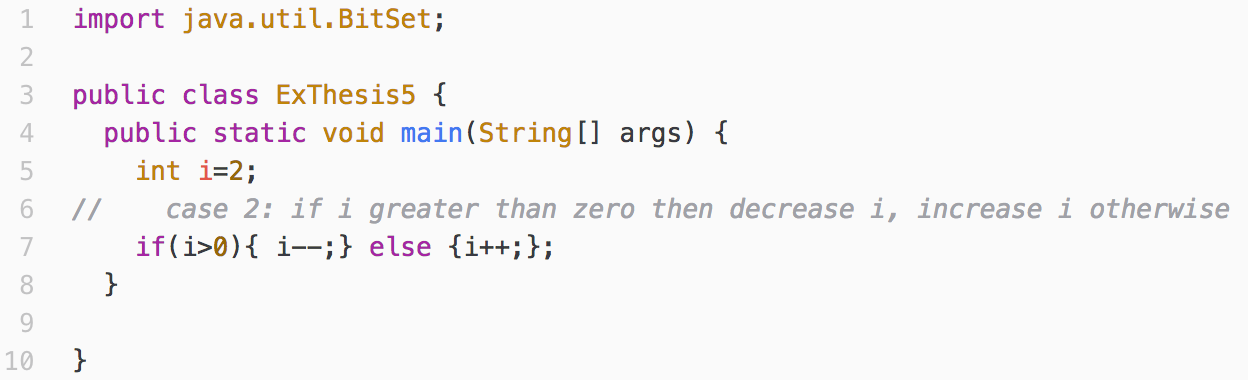
\includegraphics[width=14cm,height=5cm]{resources/fig_expressiveness_example.png}%
	%\includegraphics[width=\textwidth]{conceptdriven.eps}
	\caption[Example of Expressiveness in NL-to-PL translation]{Example of Expressiveness in NL-to-PL translation} 
	\label{fig:ExpressivenessExample}
\end{figure}
NL and PL have a very separate mechanism of managing the expressiveness in description related to control structures. An example of Expressiveness difference is shown in Figure \ref{fig_ExpressivenessExample}. In this example, the description mentioned about if and otherwise case about a boolean condition. However, in the implementation, the code for the implementation is the if-then-else structure. The order of description of statement of else branch is before the term "otherwise", while "else" keyword should be before this statement in the implementation. Along with basic control structure, we can face the problem of expressiveness in many other structure and algorithms, like loop and recursion. The different of expressiveness causes the mismatch between learning the control structure of programming language given the natural language description. 

\subsection{Phrases}
Natural Language description consists of one or more phrases. In NL to PL, each phrase may have a specific semantic  meaning related to variables and statements. Phrases can be very complex and can be ambiguous about their mapping in the PL. Several phrases can be mapped to one statement in the implementation, while several sentences can be mapped to single control structure. \\

\begin{figure}[htp]
	\centering
	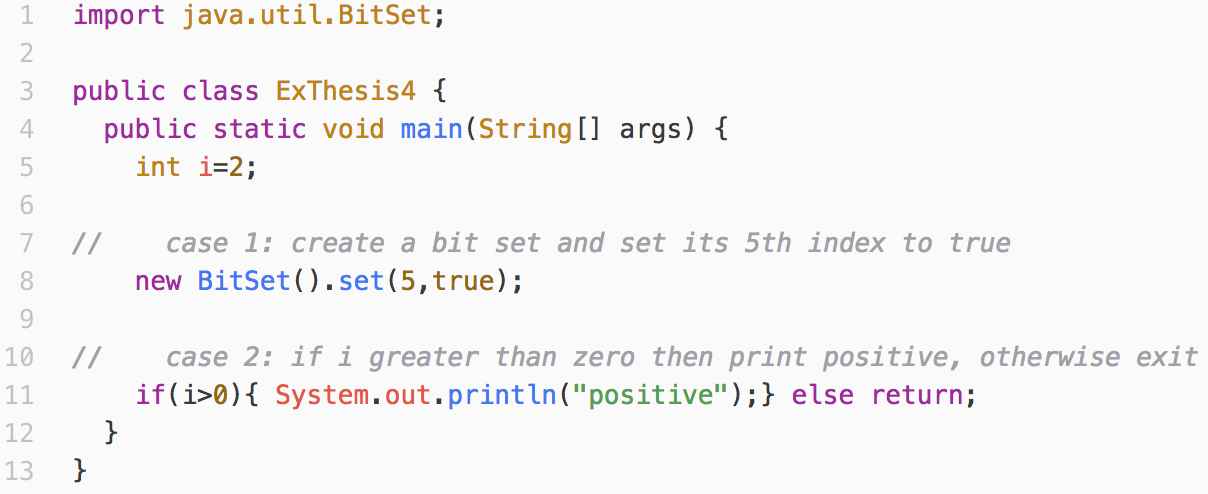
\includegraphics[width=14cm,height=6cm]{resources/fig_phrase_example.png}%
	%\includegraphics[width=\textwidth]{conceptdriven.eps}
	\caption[Example of Phrase Complexity in NL-to-PL translation]{Example of Phrase Complexity in NL-to-PL translation} 
	\label{fig:PhraseExample}
\end{figure}

In case 1 of example in Figure \ref{fig:PhraseExample}, we can see that two phrases of the description "create bit set and set its 5th index to true" corresponded to one method invocation, in which the first phrase is the receiver while the second phrase mentioned about the method identifier and expected method argument. The differences in phrase translation rules can be shown on the second case. In this example, two sentences in the documentation actually mentioned about an "If" branch and an "else" branch of an if statement. In general, the mapping of phrase to statement in NL to PL is not always be one to one mapping. The mapping rules between phrase in NL and statement in PL might depends on types of phrase along with context of NL description.
   
\subsection{Anaphoric Relations}
In natural languages, abstraction of types are not only in the form of class name like example we show in deixis but also in the form of providing description relate to class properties and methods. An example of anaphoric relations is  shown in example in Fiigure \ref{fig:AnaphoricExample}. In the NL description, a noun phrase "dog" actually refers to a class name and the verb "is barking" mentioned about method bark() defined inside a Dog class. This description implies about a validation for NL description, in which ensure that bark() has to be a method of Dog object. Depending on paradigm of programming language, the corresponding implementation may be differed. For example, in object-oriented language, we must assured that the project contains this description has definition of Dog class with bark() method, while in functional language like C or Pascal, we valid our program by finding a function bask() that accept a struct "Dog". \\

\begin{figure}[htp]
	\centering
	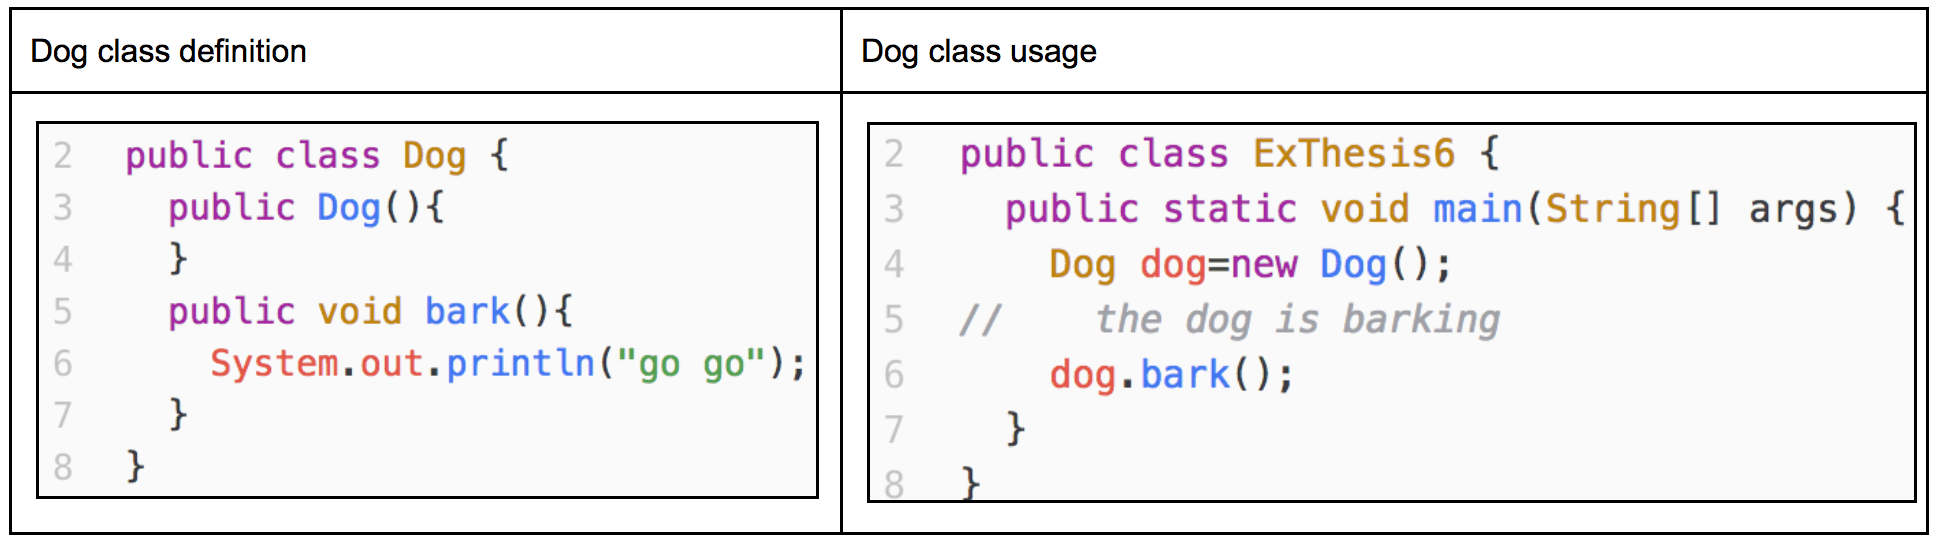
\includegraphics[width=18cm,height=6cm]{resources/fig_anaphoric_example.png}%
	%\includegraphics[width=\textwidth]{conceptdriven.eps}
	\caption[Example of Anaphoric Relation in NL-to-PL translation]{Example of Anaphoric Relation n NL-to-PL translation} 
	\label{fig:AnaphoricExample}
\end{figure}


Along with deixis, anaphoric relations provides the full support for indirect reference between NL and PL. While deixis relate to how to mention about a type information in form of class name only or pronoun, anaphoric relations focuses on expression every properties of an instance, including its methods and fields. A common of type of this relation is relation between verb to method invocation. When you see a verb in NL description along with a class name like Figure \ref{fig:AnaphoricExample}, it means that the corresponding implementation is about a method invocation of the class name in NL description.
 
\subsection{Context}
To realizing literate programming, context is an important element deciding the correctness of natural language to programming language translation. Unlike NL-to-NL translation which considered the context such as surrounding phrases or surrounding sentences given an input, the NL-to-PL considered both the natural language side and programming language side as context of given NL description. \\

Given a NL description, its related implementation might depend on surrounding NL description. In case 2 of example in Figure \ref{fig:PhraseExample}. the phrase "set its 5th index to true" has a translated result as a method invocation "set" of java.util.BitSet object. We know about the receiver of this implementation based on the previous phrase "create a bit set", which provides us information about a BitSet object. If we don't have the first phrase, we cannot inferred to the correct set method invocation, though we have method name along with parameters. \\

Along with context from NL part, information from programming language part brings an essential context for NL description. In case 2 of Figure  \ref{fig:PhraseExample}, we don't have information about the constructor of Bit Set. However, we can predict about the receiver of "set" method identifier based on the surrounding code, in which we have the information about a BitSet object. Context of PL parts provides all possible variables and class name are valid to use for the NL description. Context at PL level helps to restrict the implementation parts only relate to APIs that define in the scope of project, including its imported jar file and source code files. In our knowledge, current techniques for generating code from natural language considered the NL context as a full context and skip the information about surrounding code like AnyCode [\cite{Gvero:2015:SJE:2814270.2814295}] . In AnyCode, each NL description solved as a query for code instead of a comment, which hinders its ability for realizing literate programming, which requires NL descriptions consistent with surrounding NL context and PL context.

\subsection{Ambiguity}
Ambiguity in NL to PL translation means that one element in NL may has many interpretations, which the correct one may be varied based on the context. We can manually check to find the correct interpretation but an automatic translation engine doesn't have the ability to do that. To allow reasoning and de-ambiguous the translation result, we need to study types of ambiguity and design an algorithm for reasoning. In our knowledge, their are 2 important types of ambiguity in NL side and PL sides. \\

\begin{figure}[htp]
	\centering
	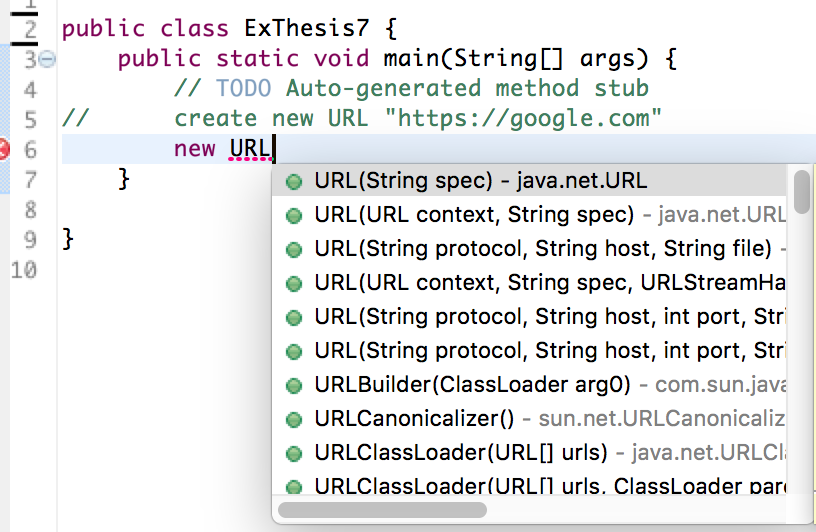
\includegraphics[width=14cm,height=6cm]{resources/fig_url_ambiguous_example.png}%
	%\includegraphics[width=\textwidth]{conceptdriven.eps}
	\caption[Example of URL type ambigous in NL-to-PL translation]{Example of URL type ambigous in NL-to-PL translation} 
	\label{fig:UrlAmbiguousExample}
\end{figure}

In NL side, noun and verb are two popular elements that have ambiguous in translated results. With noun, class name in NL might have more than one type annotation in PL. Information of correct type annotations can depend on the context of source file projects. In example show in Figure \ref{fig:UrlAmbiguousExample}, the class name "URL" has several type annotations, in which the most popular one is "java.net.URL", With verb, the ambiguity can happen between statement trigger or method invocation. In case 1 show on Figure \ref{fig:VerbAmbiguousExample}, the "set" verb is a assignment statement in the implementation, while in case 2 it is a method invocation set of Hash Map. There are several information from context can differentiate between two cases. In example one, the verb is used with a variable, a preposition "to" and a value that have the same type with a variable. In example two, the verb is used with two variable written consecutively. We can rely on such information to make correct reasoning.  \\

\begin{figure}[htp]
	\centering
	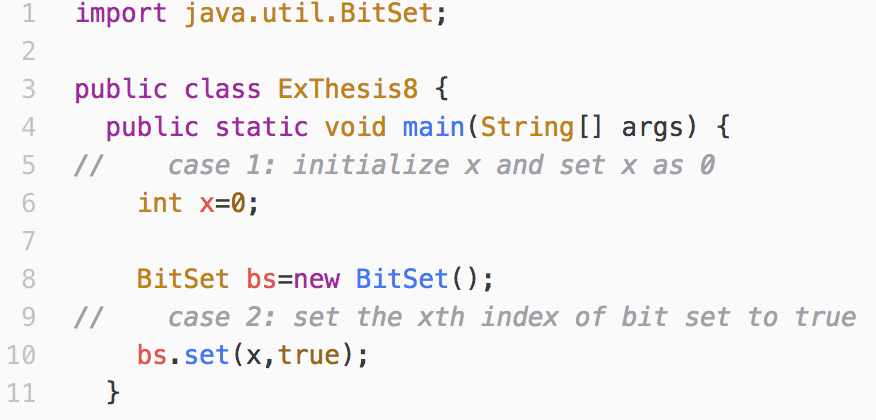
\includegraphics[width=14cm,height=6cm]{resources/fig_set_ambiguous_example.png}%
	%\includegraphics[width=\textwidth]{conceptdriven.eps}
	\caption[Example of verb ambigous in NL-to-PL translation]{Example of verb ambigous in NL-to-PL translation} 
	\label{fig:VerbAmbiguousExample}
\end{figure}

In PL side, ambiguous can happen between translating verb as method invocation. One verb can be translated to multiple invocations. In case 2 of example show in Figure \ref{}, there are in over 40 method APIs named "set" in libraries of JDK and apache common io. They have the same identifiers but their behavior are differed from each other, based on their receiver and argument. To reason the correct API for verbs, relying on the NL context including variables and value defined in the NL description might be a good direction. In overall, ambiguous is one of the most challenges for NL-to-PL translation, which make code query system like [\cite{Gvero:2015:SJE:2814270.2814295}] cannot be used for literate programming, since it doesn't use enough context in PL for reasoning the correct interpretation. 
     
\section{Elements  of a Natural Language parser}

Stanford-NLP [\cite{P13-1045}] is one of the most popular Natural Language Processing toolkits. The core of Stanford-NLP is based on its Stanford Parser. Stanford parser is a natural language parser, which analyses the grammatical structure of sentences and identifying type of words, such as verb, subject or object. Stanford Parser uses probabilistic parser, which uses information from corpus of sentences parsed manually to analyze new sentence. The output of this parser is an natural language parsed tree, which is important in NL to PL translation systems such as AnyCode [\cite{Gvero:2015:SJE:2814270.2814295}]. In this tree, each nodes will belong to one type of the Penn Treebank tags [\cite{Taylor2003}]. In this section, we study the purpose of each Treebank tags and its context in NL description for PL. In total, there are 82 tags defined in [\cite{Taylor2003}]. In these tags, 62 of them are frequently used in  NL description which are belong to 3 types: clause level, phrase level and word level. This section will introduce an overview of each NL tags.

\subsection{Clause level tags}
Clause level tags are elements for representing a grammar structure of sentences. The most frequent type of clause is the simple declarative clause which has abbreviation S. S is one of the basic clauses for conversation and writing [\cite{Cambridge:STag}]. The grammar of declarative sentence usually contains subject, verb and object. An example of S is shown in Figure \ref{fig:StagExample}. \\
\begin{figure}[htp]
	\centering
	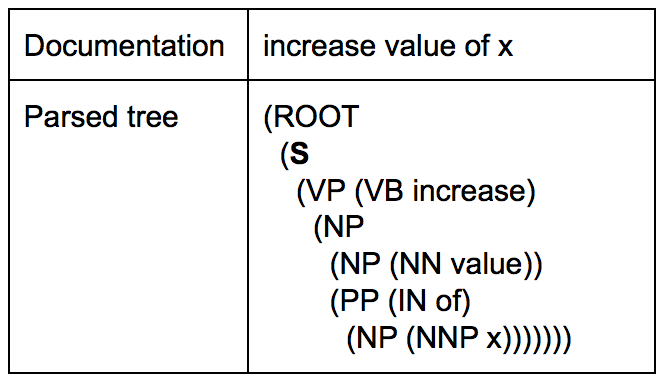
\includegraphics[width=8cm,height=4cm]{resources/fig_stag_example}
	\caption[Example of Simple declarative clause (S tag)] {Example of Simple declarative clause (S tag)}
	\label{fig:StagExample}
\end{figure}
Along with declarative sentence, NL grammar allows other types of sentences such as interrogate, imperative or exclamatory. There are 4 other types of clause defined by PennTree Bank: SBAR, SBARQ, SINV and SQ. SBAR stands for subordinate clause. It usually begin with subordinating conjunction along with a simple declarative clause. In NL description for PL, we can see SBAR frequently in the form of "if" clause. In case 1 example in Figure \ref{fig:SBARSBARQTagExample}, "if" solved as subordinating conjunction before description of boolean condition "x is greater than zero". SBARQ stands for direct question introduced by wh-word or wh-phrase. Since NL description is usually a description about behavior of implementation, SBARQ rarely see in NL to PL translation. SINV is the inverted declarative sentence, which usually has past tense verb in its content like case in example. SQ is a question that has yes/no answer options. Differ from SBARQ question, SQ sentences don't start with wh-element. Example of SBARQ tag is shown in case 2 of Figure \ref{fig:SBARSBARQTagExample}. 

\begin{figure}[htp]
	\centering
	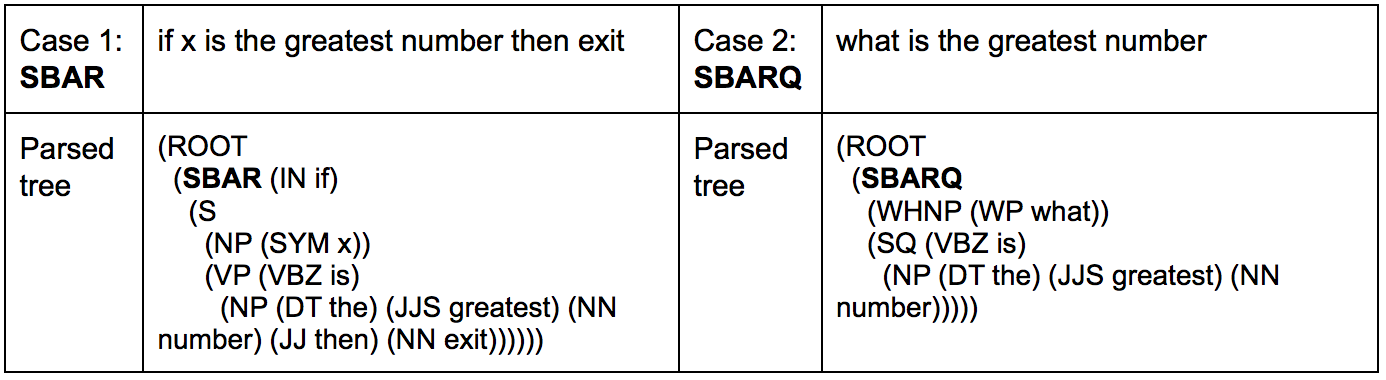
\includegraphics[width=14cm,height=4cm]{resources/fig_sbar_sbarq_2examples}
	\caption[Examples of SBAR and SBARQ tags] {Examples of SBAR and SBARQ tags}
	\label{fig:SBARSBARQTagExample}
\end{figure}

\subsection{Phrase level tags}
Phrase level tags are usually at non-terminal level of NL tree. Each types of phrase level tags consist element at leaf node as word level. In table \ref{table:SummarizeAllTags}, we show the list of phrase level tags along with examples.
\begin{longtable}{|p{.05\textwidth}|p{.15\textwidth}|p{.10\textwidth}|p{.35\textwidth}|p{.35\textwidth}|}
% Please add the following required packages to your document preamble:
% \usepackage[table,xcdraw]{xcolor}
% If you use beamer only pass "xcolor=table" option, i.e. \documentclass[xcolor=table]{beamer}

		\hline
		\rowcolor[HTML]{38FFF8} 
		\multicolumn{1}{|c|}{\cellcolor[HTML]{38FFF8}\textbf{No}} & \multicolumn{1}{c|}{\cellcolor[HTML]{38FFF8}\textbf{Level}} & \multicolumn{1}{c|}{\cellcolor[HTML]{38FFF8}\textbf{Tags}} & \multicolumn{1}{c|}{\cellcolor[HTML]{38FFF8}\textbf{Meaning in NL description}}                                 & \multicolumn{1}{c|}{\cellcolor[HTML]{38FFF8}\textbf{Example as NL description}} \\ \hline
		\rowcolor[HTML]{FFCCC9} 
		1                                                         & Clause level                                                & S                                                          & - simple declarative clause- Usually use for mention about statements                                           & increase value of x                                                             \\ \hline
		\rowcolor[HTML]{FFCCC9} 
		2                                                         & Clause level                                                & SBAR                                                       & - Clause introduced by a (possibly empty) subordinating conjunction.- Usually relate to if statement            & if x is the greatest number then exit                                           \\ \hline
		\rowcolor[HTML]{9AFF99} 
		3                                                         & Clause level                                                & SBARQ                                                      & - Direct question introduced by a wh-word or a wh-phrase.- Usually use for mentions about statements            & what is the greater number                                                      \\ \hline
		\rowcolor[HTML]{9AFF99} 
		4                                                         & Clause level                                                & SINV                                                       & - Inverted declarative sentence- Usually use for mentions about statements                                      & given to x was a value that was equal to length to array                        \\ \hline
		\rowcolor[HTML]{9AFF99} 
		5                                                         & Clause level                                                & SQ                                                         & - Inverted yes/no question- Usually relate to check condition                                                   & does x greater than zero?                                                       \\ \hline
		\rowcolor[HTML]{FFCCC9} 
		6                                                         & Phrase level                                                & ADJP                                                       & Adjective Phrase.                                                                                               & the value of x is negative.                                                     \\ \hline
		\rowcolor[HTML]{FFCCC9} 
		7                                                         & Phrase level                                                & ADVP                                                       & - Adverb Phrase.- Adverb Phrases Show How, Where, Why, When                                                     & why do we increase the value of x?                                              \\ \hline
		\rowcolor[HTML]{FFCCC9} 
		8                                                         & Phrase level                                                & CONJP                                                      & Conjunction Phrase.                                                                                             & dog and cat and fox are animals.                                                \\ \hline
		\rowcolor[HTML]{FFFFC7} 
		9                                                         & Phrase level                                                & FRAG                                                       & - Fragment (sentence that miss subjects and/or verbs).- Usually use in dialog, not so popular in NL description & From morning until night.                                                       \\ \hline
		\rowcolor[HTML]{FFFFC7} 
		10                                                        & Phrase level                                                & INTJ                                                       & - Interjection (for strong emotion) - Not popular in NL description                                             & Hello! How are you?                                                             \\ \hline
		\rowcolor[HTML]{FFFFC7} 
		11                                                        & Phrase level                                                & LST                                                        & - List marker. Includes surrounding punctuation.- Not popular in NL description                                 & 1) 2)                                                                           \\ \hline
		\rowcolor[HTML]{FFFFC7} 
		12                                                        & Phrase level                                                & NAC                                                        & - Not a Constituent- Not popular in NL description                                                              &                                                                                 \\ \hline
		\rowcolor[HTML]{FFCCC9} 
		13                                                        & Phrase level                                                & NP                                                         & - Noun Phrase.- Usually use for describe class name or variables                                                & the array is created                                                            \\ \hline
		\rowcolor[HTML]{9AFF99} 
		14                                                        & Phrase level                                                & NX                                                         & - Used within certain complex NPs to mark the head of the NP. - Not popular in NL description                   &                                                                                 \\ \hline
		\rowcolor[HTML]{9AFF99} 
		15                                                        & Phrase level                                                & PP                                                         & - Prepositional Phrase.- Usually connect words between APIs or variables                                        & read value from console                                                         \\ \hline
		\rowcolor[HTML]{9AFF99} 
		16                                                        & Phrase level                                                & PRN                                                        & - Parenthetical.                                                                                                & x (the integer value) is initialized                                            \\ \hline
		\rowcolor[HTML]{9AFF99} 
		17                                                        & Phrase level                                                & PRT                                                        & - Particle- Use with little or no meaning                                                                       & move the chess up one position                                                  \\ \hline
		\rowcolor[HTML]{9AFF99} 
		18                                                        & Phrase level                                                & QP                                                         & - Quantifier Phrase; used within NP.- Might use for describe loop                                               & every ten minutes, this method runs in a thread.                                \\ \hline
		\rowcolor[HTML]{FFFFC7} 
		19                                                        & Phrase level                                                & RRC                                                        & - Reduced Relative Clause.- Not popular in NL description                                                       & the variable we created will be used in the future.                             \\ \hline
		\rowcolor[HTML]{FFFFC7} 
		20                                                        & Phrase level                                                & UCP                                                        & - Unlike Coordinated Phrase.- Not popular in NL description.                                                    &                                                                                 \\ \hline
		\rowcolor[HTML]{FFCCC9} 
		21                                                        & Phrase level                                                & VP                                                         & - Verb Phrase.- Usually use for represent statements, operations and method invocations.                        & increase value of x                                                             \\ \hline
		\rowcolor[HTML]{9AFF99} 
		22                                                        & Phrase level                                                & WHADJP                                                     & Wh-adjective Phrase                                                                                             & how does it work                                                                \\ \hline
		\rowcolor[HTML]{9AFF99} 
		23                                                        & Phrase level                                                & WHAVP                                                      & Wh-adverb Phrase.                                                                                               & why do I increase x                                                             \\ \hline
		\rowcolor[HTML]{9AFF99} 
		24                                                        & Phrase level                                                & WHNP                                                       & Wh-noun Phrase.                                                                                                 & we calculate how many candies in a box.                                         \\ \hline
		\rowcolor[HTML]{9AFF99} 
		25                                                        & Phrase level                                                & WHPP                                                       & Wh-prepositional Phrase. Prepositional phrase containing a wh-noun phrase.                                      & we create a console then we get the value of x from which.                      \\ \hline
		\rowcolor[HTML]{FFFFC7} 
		26                                                        & Phrase level                                                & X                                                          & - Unknown, uncertain, or unbracketable.- Not popular in NL description.                                         &                                                                                 \\ \hline
		\rowcolor[HTML]{FFCCC9} 
		27                                                        & Word level                                                  & CC                                                         & coordinating conjunction                                                                                        & and                                                                             \\ \hline
		\rowcolor[HTML]{9AFF99} 
		28                                                        & Word level                                                  & CD                                                         & cardinal number                                                                                                 & 1, third                                                                        \\ \hline
		\rowcolor[HTML]{9AFF99} 
		29                                                        & Word level                                                  & DT                                                         & determiner                                                                                                      & the                                                                             \\ \hline
		\rowcolor[HTML]{9AFF99} 
		30                                                        & Word level                                                  & EX                                                         & existential there                                                                                               & there is                                                                        \\ \hline
		\rowcolor[HTML]{9AFF99} 
		31                                                        & Word level                                                  & FW                                                         & foreign word                                                                                                    & les                                                                             \\ \hline
		\rowcolor[HTML]{9AFF99} 
		32                                                        & Word level                                                  & IN                                                         & preposition, subordinating conjunction                                                                          & in, of, like                                                                    \\ \hline
		\rowcolor[HTML]{9AFF99} 
		33                                                        & Word level                                                  & IN/that                                                    & that as subordinator                                                                                            & that                                                                            \\ \hline
		\rowcolor[HTML]{9AFF99} 
		34                                                        & Word level                                                  & JJ                                                         & adjective                                                                                                       & green                                                                           \\ \hline
		\rowcolor[HTML]{9AFF99} 
		35                                                        & Word level                                                  & JJR                                                        & adjective, comparative                                                                                          & greener                                                                         \\ \hline
		\rowcolor[HTML]{9AFF99} 
		36                                                        & Word level                                                  & JJS                                                        & adjective, superlative                                                                                          & greenest                                                                        \\ \hline
		\rowcolor[HTML]{9AFF99} 
		37                                                        & Word level                                                  & LS                                                         & list marker                                                                                                     & 1)                                                                              \\ \hline
		\rowcolor[HTML]{9AFF99} 
		38                                                        & Word level                                                  & MD                                                         & modal                                                                                                           & could, will                                                                     \\ \hline
		\rowcolor[HTML]{FFCCC9} 
		39                                                        & Word level                                                  & NN                                                         & noun, singular or mass                                                                                          & table                                                                           \\ \hline
		\rowcolor[HTML]{FFCCC9} 
		40                                                        & Word level                                                  & NNS                                                        & noun plural                                                                                                     & tables                                                                          \\ \hline
		\rowcolor[HTML]{FFCCC9} 
		41                                                        & Word level                                                  & NNP                                                        & proper noun, singular                                                                                           & David                                                                           \\ \hline
		\rowcolor[HTML]{FFCCC9} 
		42                                                        & Word level                                                  & NNPS                                                       & proper noun, plural                                                                                             & Iowans                                                                          \\ \hline
		\rowcolor[HTML]{FFFFC7} 
		43                                                        & Word level                                                  & PDT                                                        & predeterminer                                                                                                   & both the variables                                                              \\ \hline
		\rowcolor[HTML]{FFFFC7} 
		44                                                        & Word level                                                  & POS                                                        & possessive ending                                                                                               & friend’s                                                                        \\ \hline
		\rowcolor[HTML]{9AFF99} 
		45                                                        & Word level                                                  & PP                                                         & personal pronoun                                                                                                & I, he, it                                                                       \\ \hline
		\rowcolor[HTML]{FFFFC7} 
		46                                                        & Word level                                                  & PP\$                                                       & possessive pronoun                                                                                              & my, his                                                                         \\ \hline
		\rowcolor[HTML]{9AFF99} 
		47                                                        & Word level                                                  & RB                                                         & adverb                                                                                                          & however, usually, naturally, here, good                                         \\ \hline
		\rowcolor[HTML]{9AFF99} 
		48                                                        & Word level                                                  & RBR                                                        & adverb, comparative                                                                                             & better                                                                          \\ \hline
		\rowcolor[HTML]{9AFF99} 
		49                                                        & Word level                                                  & RBS                                                        & adverb, superlative                                                                                             & best                                                                            \\ \hline
		\rowcolor[HTML]{9AFF99} 
		50                                                        & Word level                                                  & RP                                                         & particle                                                                                                        & give up                                                                         \\ \hline
		\rowcolor[HTML]{9AFF99} 
		51                                                        & Word level                                                  & SENT                                                       & Sentence-break punctuation                                                                                      & . ! ?                                                                           \\ \hline
		\rowcolor[HTML]{9AFF99} 
		52                                                        & Word level                                                  & SYM                                                        & Symbol                                                                                                          & / {[} = *                                                                       \\ \hline
		\rowcolor[HTML]{9AFF99} 
		53                                                        & Word level                                                  & TO                                                         & infinitive ‘to’                                                                                                 & togo                                                                            \\ \hline
		\rowcolor[HTML]{FFCCC9} 
		54                                                        & Word level                                                  & VB                                                         & verb be, base form                                                                                              & be                                                                              \\ \hline
		\rowcolor[HTML]{FFCCC9} 
		55                                                        & Word level                                                  & VBD                                                        & verb be, past tense                                                                                             & was, were                                                                       \\ \hline
		\rowcolor[HTML]{FFCCC9} 
		56                                                        & Word level                                                  & VBG                                                        & verb be, gerund/present participle                                                                              & being                                                                           \\ \hline
		\rowcolor[HTML]{FFCCC9} 
		57                                                        & Word level                                                  & VBN                                                        & verb be, past participle                                                                                        & been                                                                            \\ \hline
		\rowcolor[HTML]{FFCCC9} 
		58                                                        & Word level                                                  & VBP                                                        & verb be, sing. present, non-3d                                                                                  & am, are                                                                         \\ \hline
		\rowcolor[HTML]{FFCCC9} 
		59                                                        & Word level                                                  & VBZ                                                        & verb be, 3rd person sing. present                                                                               & is                                                                              \\ \hline
		\rowcolor[HTML]{9AFF99} 
		60                                                        & Word level                                                  & VH                                                         & verb have, base form                                                                                            & have                                                                            \\ \hline
		\rowcolor[HTML]{9AFF99} 
		61                                                        & Word level                                                  & VHD                                                        & verb have, past tense                                                                                           & had                                                                             \\ \hline
		\rowcolor[HTML]{9AFF99} 
		62                                                        & Word level                                                  & VHG                                                        & verb have, gerund/present participle                                                                            & having                                                                          \\ \hline
		\rowcolor[HTML]{9AFF99} 
		63                                                        & Word level                                                  & VHN                                                        & verb have, past participle                                                                                      & had                                                                             \\ \hline
		\rowcolor[HTML]{9AFF99} 
		64                                                        & Word level                                                  & VHP                                                        & verb have, sing. present, non-3d                                                                                & have                                                                            \\ \hline
		\rowcolor[HTML]{9AFF99} 
		65                                                        & Word level                                                  & VHZ                                                        & verb have, 3rd person sing. present                                                                             & has                                                                             \\ \hline
		\rowcolor[HTML]{9AFF99} 
		66                                                        & Word level                                                  & VV                                                         & verb, base form                                                                                                 & take                                                                            \\ \hline
		\rowcolor[HTML]{9AFF99} 
		67                                                        & Word level                                                  & VVD                                                        & verb, past tense                                                                                                & took                                                                            \\ \hline
		\rowcolor[HTML]{9AFF99} 
		68                                                        & Word level                                                  & VVG                                                        & verb, gerund/present participle                                                                                 & taking                                                                          \\ \hline
		\rowcolor[HTML]{9AFF99} 
		69                                                        & Word level                                                  & VVN                                                        & verb, past participle                                                                                           & taken                                                                           \\ \hline
		\rowcolor[HTML]{9AFF99} 
		70                                                        & Word level                                                  & VVP                                                        & verb, sing. present, non-3d                                                                                     & take                                                                            \\ \hline
		\rowcolor[HTML]{9AFF99} 
		71                                                        & Word level                                                  & VVZ                                                        & verb, 3rd person sing. present                                                                                  & takes                                                                           \\ \hline
		\rowcolor[HTML]{9AFF99} 
		72                                                        & Word level                                                  & WDT                                                        & wh-determiner                                                                                                   & which                                                                           \\ \hline
		\rowcolor[HTML]{9AFF99} 
		73                                                        & Word level                                                  & WP                                                         & wh-pronoun                                                                                                      & who, what                                                                       \\ \hline
		\rowcolor[HTML]{9AFF99} 
		74                                                        & Word level                                                  & WP\$                                                       & possessive wh-pronoun                                                                                           & whose                                                                           \\ \hline
		\rowcolor[HTML]{9AFF99} 
		75                                                        & Word level                                                  & WRB                                                        & wh-abverb                                                                                                       & where, when                                                                     \\ \hline
        
        \caption[Semantic explanation of Penn-Tree Bank tags]{Semantic explanation of Penn-Tree Bank tags and  their popularity in NL description (red block as popular, green block as normally and yellow block as rarely used)}
       \label{table:SummarizeAllTags} 
\end{longtable}

\subsection{Word level tags}
Clause level tags are node at terminal level in NL tree. The list of each word level tags and example are shown in table \ref{table:SummarizeAllTags}. 
In NL to PL translation, noun, verb preposition and conjunction are the most important tags used for NL description. Noun group usually represents for class name and variables, with plural or non-plural. Verb are used as statement trigger or method invocation description.Preposition is usually used as the connector between variables in the context of arguments in a method invocation, while conjunction responds to the connection between phrase in NL. Group of adjective and adverb are usually used for representing properties of a class or an object instance.

